\chapter{The Limits of Direct Reinforcement Learning of Decision Tree Policies}
In this chapter we investigate the properties of reinforcement learning for learning a depth-1 decision tree policy for a very simple Markov decision process.
Using the formal framework of partially observable iterative bounding Markvov decision processes (cite), we aim to learn partially observable deterministic policies that correspond to decision tree policies (cite).

We will attempt to learn a depth-1 tree policy for the $2\times 2$ grid world from (cite) as the base MDP by soving the example POIBMDP from the previous chapter.
To focus on reinforcement learning properties in POIBMDPs rather than, e.g., modelling properties, we will carefully craft POIBMDPs such that the \textit{optimal} partially observable deterministic policy corresponds to a depth-1 tree policy.
To do so, we present next how the POIBMDP objective values (cite) from different decision tree policies change with $\zeta$ for some fixed discount factor $\gamma$.  

\section{Constructing POIBMDPs which optimal solutions are the depth-1 tree}
\begin{figure}[htbp]
    \centering
    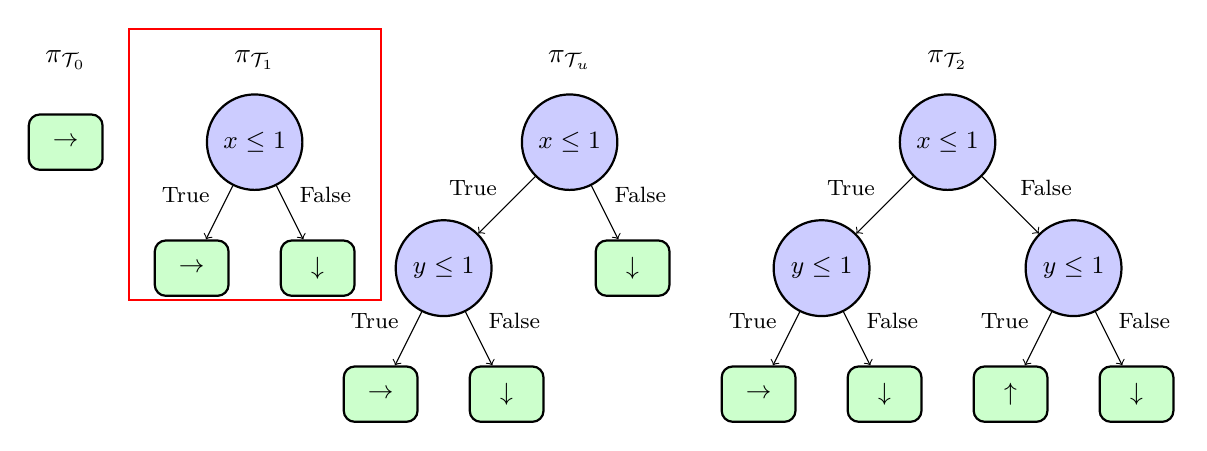
\begin{tikzpicture}[
        scale=0.8,
        decision/.style={circle, draw, thick, fill=blue!20, text width=2.5em, text centered, minimum height=2.5em, font=\small},
        leaf/.style={rectangle, draw, thick, fill=green!20, text width=2em, text centered, rounded corners, minimum height=2em, font=\small},
        edge_label/.style={font=\footnotesize, midway}
    ]
        
        \node[leaf] at (-3, 0) {$\rightarrow$};
        % Tree 4: if x <= 0.5 move right else move left
        \node[decision] (tree4_root) at (0,0) {$x \leq 1$};
        \node[leaf] (tree4_right) at (-1,-2) {$\rightarrow$};
        \node[leaf] (tree4_left) at (1,-2) {$\downarrow$};
        \draw[->] (tree4_root) -- (tree4_right) node[edge_label, above left] {True};
        \draw[->] (tree4_root) -- (tree4_left) node[edge_label, above right] {False};
        
        % Draw a square around the tree
        \draw[thick, red] (-2, 1.8) rectangle (2, -2.5);

        % Tree 7: if x <= 0.5 and y <= 0.5 move right else move down
        \node[decision] (tree7_root) at (5,0) {$x \leq 1$};
        \node[decision] (tree7_y) at (3,-2) {$y \leq 1$};
        \node[leaf] (tree7_right) at (2,-4) {$\rightarrow$};
        \node[leaf] (tree7_down) at (4,-4) {$\downarrow$};
        \node[leaf] (tree7_down2) at (6,-2) {$\downarrow$};
        \draw[->] (tree7_root) -- (tree7_y) node[edge_label, above left] {True};
        \draw[->] (tree7_root) -- (tree7_down2) node[edge_label, above right] {False};
        \draw[->] (tree7_y) -- (tree7_right) node[edge_label, above left] {True};
        \draw[->] (tree7_y) -- (tree7_down) node[edge_label, above right] {False};


        \node[decision] (tree7_root) at (11,0) {$x \leq 1$};
        \node[decision] (tree7_y) at (9,-2) {$y \leq 1$};
        \node[decision] (tree7_y2) at (13,-2) {$y \leq 1$};
        \node[leaf] (tree7_right) at (8,-4) {$\rightarrow$};
        \node[leaf] (tree7_down) at (10,-4) {$\downarrow$};
        \node[leaf] (tree7_right2) at (12,-4) {$\uparrow$};
        \node[leaf] (tree7_down2) at (14,-4) {$\downarrow$};
        \draw[->] (tree7_root) -- (tree7_y) node[edge_label, above left] {True};
        \draw[->] (tree7_root) -- (tree7_y2) node[edge_label, above right] {False};
        \draw[->] (tree7_y) -- (tree7_right) node[edge_label, above left] {True};
        \draw[->] (tree7_y) -- (tree7_down) node[edge_label, above right] {False};
        \draw[->] (tree7_y2) -- (tree7_right2) node[edge_label, above left] {True};
        \draw[->] (tree7_y2) -- (tree7_down2) node[edge_label, above right] {False};

        % Labels
        \node[above] at (-3,1) {$\pi_{\mathcal{T}_0}$};
        \node[above] at (0,1) {$\pi_{\mathcal{T}_1}$};
        \node[above] at (5,1) {$\pi_{\mathcal{T}_u}$};
        \node[above] at (11,1) {$\pi_{\mathcal{T}_2}$};


    \end{tikzpicture}
    \caption{For each decision tree structure, e.g., depth-1 or unbalanced depth-2, in the space of deterministic partially observable POIBMDP policies, we illustrate the decision tree which gets the highest base rewards.}
    \label{fig:optimal-policy-trees}
\end{figure}

In this section we compute the \textit{exact} objective values of POIBMDP policies as functions of $\zeta$. AFter doing so, we can look for $\zeta$ values such that the optimal POIBMDP policy corresponds to a depth-1 decision tree for the grid world MDP from the previous chapter.  
Indeed, because we know all the base states, all the observations, all the actions, all the rewards and all the transitions, we can compute exactly the values of different partially observable deterministic policies given $\zeta$ the reward for IGAs and $\gamma$ the discount factor.

Each of those policies can be one of the following trees illustrated in Figure (cite): 
\begin{itemize}
    \item $\pi_{\mathcal{T}_0}$: a depth-0 tree equivalent to always taking the same base action 
    \item $\pi_{\mathcal{T}_1}$: a depth-1 tree equivalent alternating between an IGA and a base action 
    \item $\pi_{\mathcal{T}_u}$: an unbalanced depth-2 tree that sometimes takes two IGAs then a base action and sometimes a an IGA then a base action
    \item $\pi_{\mathcal{T}_2}$: a depth-2 tree that alternates between taking two IGAs and a base action
    \item an inifinite ``tree'' that only takes IGAs
\end{itemize}
Furthermore, because from (cite) we know that for POMDPs, stochastic policies can sometimes be optimal, we also compute the value of the stochastic policy that alternates between two base actions: $\rightarrow$ and $\downarrow$.
Those two base actions always lead to the goal state in expectation.

We detail the calculations for the detpth-1 decision tree objective value (cite) and defer the calculations for the other policies to the Appendix (cite).

\begin{proposition}[Depth-1 decision tree objective value] The objective value of the best depth-1 decision tree from Figure (cite) is $V^{\pi_{\mathcal{T}_1}}(o_0) = \frac{4\zeta + \gamma + 2\gamma^3 + \gamma^5}{4(1-\gamma^2)}$.
\end{proposition}

\begin{proof} $\pi_{\mathcal{T}_1}$ has one root node that tests $x\leq1$ (respectively $y\leq1$) and two leaf nodes $\rightarrow$ and $\downarrow$. 
To compute $V^\pi_{\mathcal{T}_1}(o_0)$, we compute the values of $\pi_{\mathcal{T}_1}$ in each of the possible startin states $(s_0, o_0), (s_1, o_0), (s_2, o_0), (s_g, o_0)$ and compute the expectation over those. 
At inititalization, when the base state is $s_g = (1.5, 0.5)$, the depth-1 decision tree policy cycles between taking an information gathering action $x\leq1$ and moving down to get a positive reward for which it gets the returns:
\begin{align*}
    V^{\pi_{\mathcal{T}_1}} (s_g, o_0) &= \zeta + \gamma + \gamma^2 \zeta + \gamma^3 \dots \\
    &= \overset{\infty}{\underset{t=0}\sum} \gamma^{2t} \zeta + \overset{\infty}{\underset{t=0}\sum} \gamma^{2t+1} \\
    &= \frac{\zeta + \gamma}{1 - \gamma^2}
\end{align*}
At inititialization, in either of the base states $s_0=(0.5,0.5)$ and $s_2=(1.5, 1.5)$, the value of the depth-1 decision tree policy is the return when taking one information gathering action $x\leq1$, then moving right or down, then following the policy from the goal state $s_g$:
\begin{align*}
    V^{\pi_{\mathcal{T}_1}} (s_0, o_0) &= \zeta + \gamma 0 + \gamma^2 V^{\pi_{\mathcal{T}_1}} (s_g, o_0) \\
    &= \zeta + \gamma^2 V^{\pi_{\mathcal{T}_1}} (s_g, o_0) \\
    &= V^{\pi_{\mathcal{T}_1}} (s_2, o_0)
\end{align*}
Similarly, the value of the best depth-1 decision tree policy in state $s_1=(0.5,1.5)$ is the value of taking one information gathering action then moving right to $s_2$ then following the policy in $s_2$:
\begin{align*}
    V^{\pi_{\mathcal{T}_1}} (s_1, o_0) &= \zeta + \gamma 0 + \gamma^2 V^{\pi_{\mathcal{T}_1}} (s_2, o_0) \\
    &= \zeta + \gamma^2 V^{\pi_{\mathcal{T}_1}} (s_2, o_0) \\
    &= \zeta + \gamma^2 (\zeta + \gamma^2 V^{\pi_{\mathcal{T}_1}} (s_g, o_0)) \\
    &= \zeta + \gamma^2 \zeta + \gamma^4 V^{\pi_{\mathcal{T}_1}} (s_g, o_0)
\end{align*}
Since the probability of being in any base states at initialization given that the agent observe $o_0$ is the probability of being in any base states at initialization, we can write:
\begin{align*}
    V^{\pi_{\mathcal{T}_1}} (o_0) &= \frac{1}{4} V^{\pi_{\mathcal{T}_1}} (s_g, o_0) + \frac{2}{4} V^{\pi_{\mathcal{T}_1}} (s_2, o_0) + \frac{1}{4} V^{\pi_{\mathcal{T}_1}} (s_1, o_0) \\
    &= \frac{1}{4} \frac{\zeta + \gamma}{1 - \gamma^2} + \frac{2}{4} (\zeta + \gamma^2 \frac{\zeta + \gamma}{1 - \gamma^2}) + \frac{1}{4} (\zeta + \gamma^2 \zeta + \gamma^4 \frac{\zeta + \gamma}{1 - \gamma^2}) \\
    &= \frac{1}{4} \frac{\zeta + \gamma}{1 - \gamma^2} + \frac{2}{4} (\frac{\zeta + \gamma ^ 3}{1-\gamma^2}) + \frac{1}{4}(\frac{\zeta+\gamma^5}{1-\gamma^2}) \\
    &= \frac{4\zeta + \gamma + 2\gamma^3 + \gamma^5}{4(1-\gamma^2)}
\end{align*}
\end{proof}


\begin{figure}
    \centering
    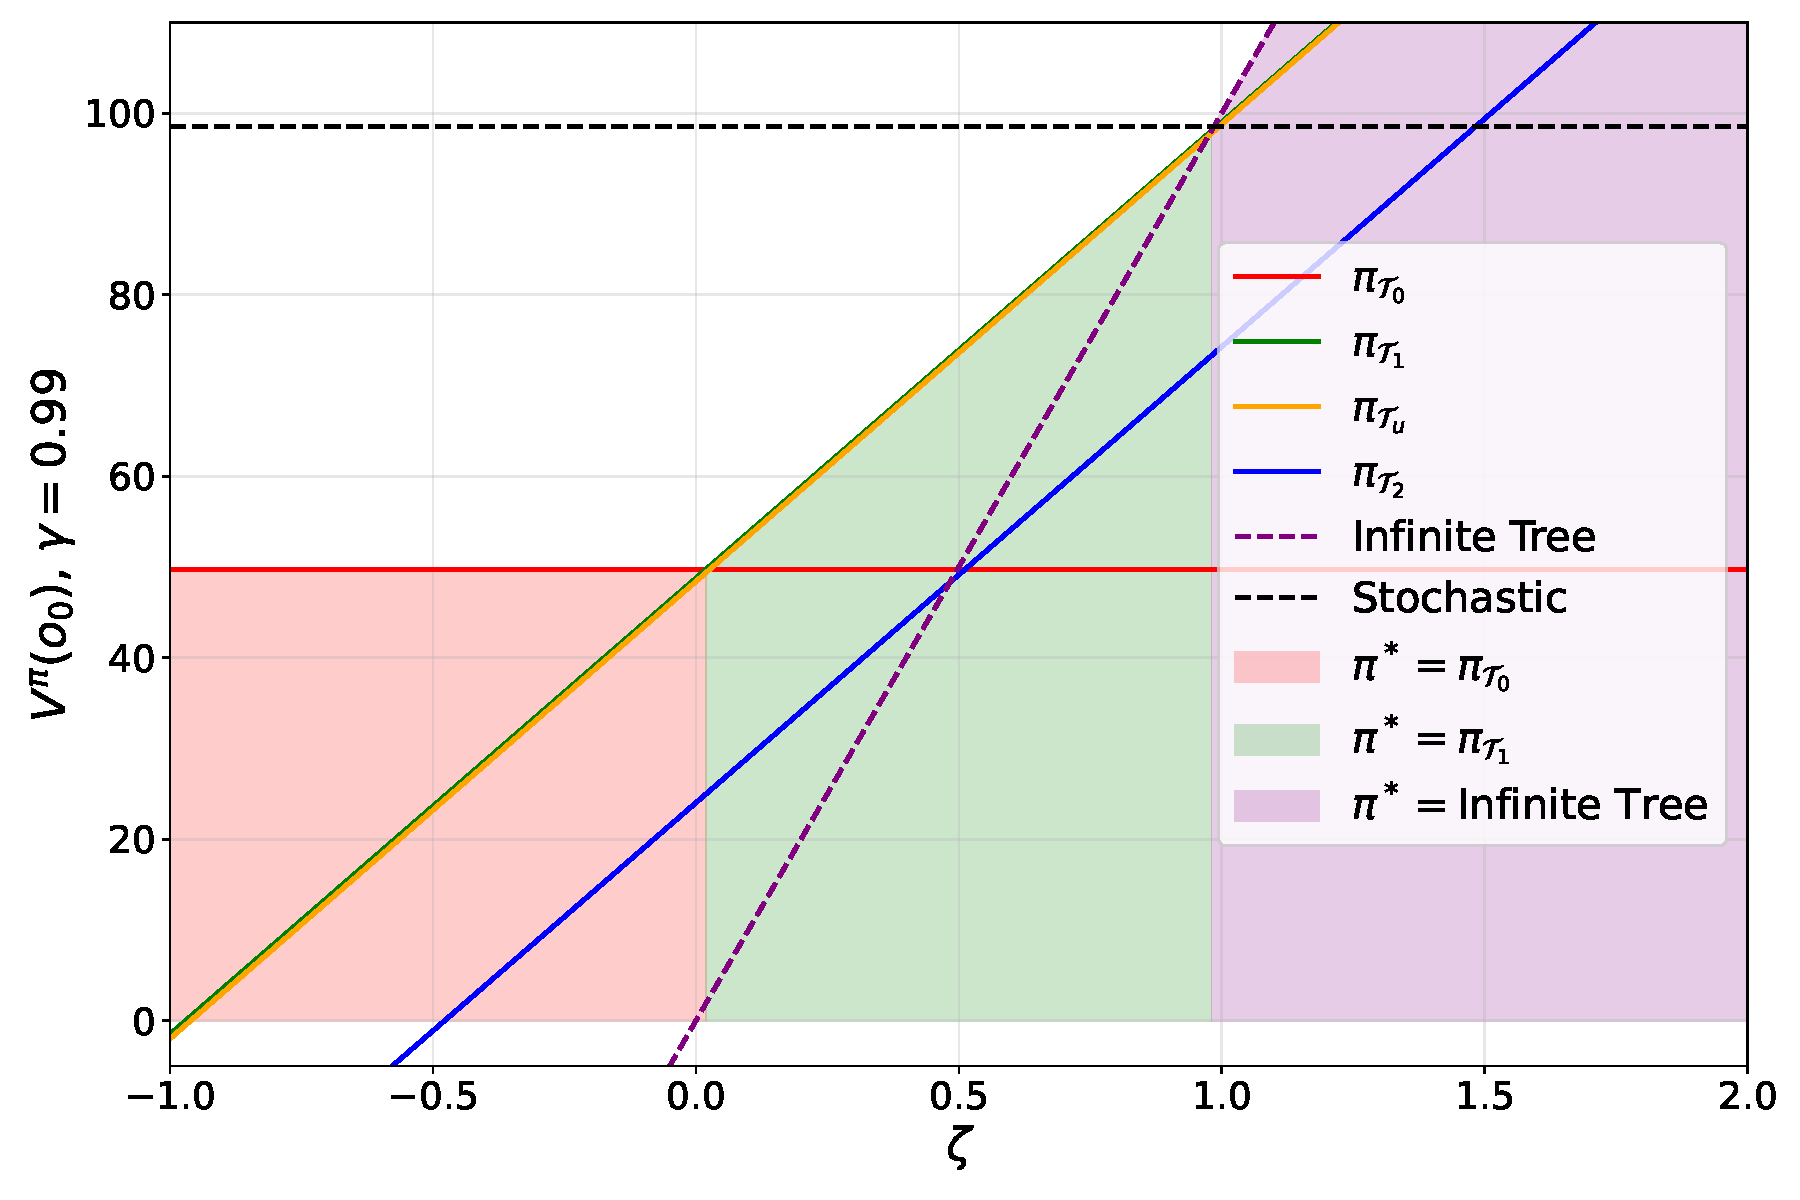
\includegraphics[width=1\textwidth]{images/images_part1/objective_values_plot.pdf}
    \caption{POIBMDP objective values of different policies as functions of $\zeta$. Shaded areas show the optimal policies in different ranges of $\zeta$ values.}\label{fig:objectives}
\end{figure}

We can now plot the POIBMDP objective values of the different policies corresponding to trees for the grid world MDP as functions of $\zeta$ when we fix $\gamma=0.99$. 
When $\gamma=0.99$, despite objective values being very similar for the depth-1 and unbalanced depth-2 tree, we now know that {\color{blue}a depth-1 tree is the optimal deterministic partially observable POIBMDP policy for $0< \zeta < 1$}.

Interestingly, two POMDP challenges described in (cite) can also be observed in Figure (cite). 
First, there is a whole range of $\zeta$ values for which the stochastic policy is optimal.
Second, for e.g. $\zeta=0.5$, while the depth-1 tree is the optimal deterministic partially observable policy, the value of state $(s_2, o_0) = (1.5, 1.5, 0, 2, 0, 2)$ is not maximized by this policy but by the sub-optimal policy that always goes down.

Now that we know to what values to set $\zeta$ in our POIBMDPs, we can apply reinforcement learning algorithms to learn partially observable deterministic policies corresponding to the optimal depth-1 decision tree.

\section{Results}

Unfortunately, our results are negative and show that reinforcement learning fails for the aforementioned problem. Let us understand why.

\subsection{Experimental Setup}

\paragraph{Baselines:} we consider two groups of RL algorithms. The first group is standard tabular RL naively applied to POIBMDPs; Q-learning (cite)(cite), Sarsa (cite)(cite), and Policy Gradient (cite)(cite).
(cite) and (cite) already studied the theoretical and practical implications of applying standard RL directly to POMDP by considering that partial observations are full MDP states.
(cite) proved that Q-Learning will converge but without optimality guarantees. 
(cite) showed empirically that Sarsa-$\lambda$ (cite), a version of Sarsa with some sort of memory, can learn good deterministic solutions to POMDP which makes it a good candiate for our problem.

We also use a vanilla tabular Policy Gradient baseline (cite) with softmax policy, which to the best of our knowledge, nobody studied in our setting.
In theory the Policy Gradient algorithm should not be a good candidate for our problem since it searches for stochastic policies that we showed can be better than our seeked depth-1 decision tree policy (c.f. Figure (cite)).

More recently, RL algorithms were developped specially for learning policies in POMDPs. Those algorithms are called asymmetric RL which authors of the original IBMDP paper (cite) use without knowing. 
Asymmetric algorithms leverage the fact that, even if the deployed policy should depend only on partial observation, nothing forbids the use of full state information during training if the latter is available.
Asymmetric Q-learning (cite) makes use of full-state-action value function $U:S\times O \timesA \rightarrow \mathbb{R}$ to use as a temporal difference error target (cite) when updating the $Q:O\times A\rightarrow \mathbb{R}$ of intereset. 
In Algorithm (cite), we write the Asymmetric Q-learning algorithm.    

In addition to the traditional tabular RL algorithms, we also apply Asymmetric Q-learning and Asymmetric Sarsa and JSJ, the tabular algorithm from (cite)(cite) which is equivalent to a tabular Asymmetric Policy Gradient algorithm.

We use at least 200 000 time steps to train each agent. Each agent is trained on 100 seeds on each POIBMDP.  

\RestyleAlgo{ruled}
\SetKwComment{Comment}{}{}
\begin{algorithm}
    \KwData{POMDP $\mathcal{M}_{po} = \langle X, O, A, R, T, T_0, \Omega \rangle$, learning rates $\alpha_u,\quad \alpha_q$, exploration rate $\epsilon$}
    \KwResult{$\pi:O\rightarrow A$}
    Initialize $U(x,a) = 0$ for all $x \in X, a \in A$ \\
    Initialize $Q(o,a) = 0$ for all $o \in O, a \in A$ \\

    \For{each episode}{
        Initialize state $x_0 \sim T_0$ \\
        Initialize observation $o_0 \sim \Omega(x_0)$ \\

        \For{each step $t$}{
            Choose action $a_t$ using $\epsilon$-greedy: $a_t = \arg\max_a Q(o_t,a)$ with prob. $1-\epsilon$ \\
            Take action $a_t$, observe $r_t = R(x_t,a_t)$, $x_{t+1} \sim T(x_t,a_t)$, and $o_{t+1} \sim \Omega(x_{t+1})$ \\
            $y \leftarrow r + \gamma U(x_{t+1}, \argmax_{a'} Q(o_{t+1}, a'))$ \Comment{// TD target} \\
            $U(x_t,a_t) \leftarrow (1 - \alpha_u) U(x_t, a_t) + \alpha_u y $ \\
            $Q(o_t,a_t) \leftarrow (1 - \alpha_q) Q(o_t, a_t) + \alpha_q y $ \\
            $x_t \leftarrow x_{t+1}$ \\
            $o_t \leftarrow o_{t+1}$ \\
        }
    }
    $\pi(o) = \arg\max_a Q(o,a)$ \Comment{// Extract greedy policy}
    \caption{Asymmetric Q-Learning (cite)}\label{alg:asymqlearning}
\end{algorithm}

\RestyleAlgo{ruled}
\SetKwComment{Comment}{}{}
\begin{algorithm}
    \KwData{POMDP $\mathcal{M}_{po} = \langle X, O, A, R, T, T_0, \Omega \rangle$, learning rate $\alpha$, policy parameters $\theta$, number of trajectories $N$}
    \KwResult{Stochastic partially observable policy $\pi_\theta: O\rightarrow \Delta A$}
    Initialize policy parameters $\theta$ \\
    Initialize $Q(o, a) = 0$ for all observations $o$ and actions $a$ \\
    \For{each episode}{
        \For{$i = 1$ to $N$}{
            Generate trajectory $\tau_i = (s_0, a_0, r_0, s_1, a_1, r_1, \ldots, s_T)$ following $\pi_\theta$ \\
            \For{each timestep $t$ in trajectory $\tau_i$}{
                $G_t \leftarrow \sum_{k=t}^{T} \gamma^{k-t} r_k$ \Comment{// Compute return}
                Store $(o_t, a_t, G_t)$ for later averaging
            }
        }
        \For{each unique observation-action pair $(o, a)$}{
            $Q(o, a) \leftarrow \frac{1}{|\{(o, a)\}|} \sum_{(o, a, G)} G$ \Comment{// Monte Carlo estimate}
        }
        \For{each observation $o$}{
            \For{each action $a$}{
                $\pi_1(a|o) \leftarrow 1.0$ if $a = \argmax_{a'} Q(o, a')$, $0.0$ otherwise \Comment{// Deterministic policy from Q-values}
                $\pi(a|o) \leftarrow (1 - \alpha) \pi(a|o) + \alpha \pi_1(a|o)$ \Comment{// Policy improvement step}
            }
        }
        Reset $Q(o, a) = 0$ for all observations $o$ and actions $a$ \Comment{// Reset for next episode}
    }
    \caption{JSJ algorithm. Uses Monte Carlo estimates of the average reawrd value functions to perform policy imporvements (cite)}\label{alg:jsj}
\end{algorithm}

\paragraph{Hyperparameters:} For all baselines we use, when applicable, exploration rates $\epsilon=0.3$ and learning rates $\alpha=0.1$.

\paragraph{Metrics:} we will consider two metrics.
First, the sub-optimality gap of the learned policy POIBMDP value with respect to the optimal deterministic partially observable POIBMP policy: $|V^\pi^{\star}(o_0) - V^\pi(o_0)|$
Because we know the whole POIBMDP model that we can represent exactly as tables; and because we know for each $\zeta$ value the POIBMDP objective value of the optimal partially observable policy (c.f. Figure); we can report the \textit{exact} sub-optimality gaps.

Second, we consider the distribution of the learned trees structure over the 100 training seeds.
Indeed, since for every POIBMDP we train each baseline 100 times, we obtain 100 partially observable deterministic policies from which we can extract the equivalent 100 decision tree policies using Algorithm (cite).
This helps understand which trees RL tend to learn.

\subsection{Can RL baselines solve POIBMDPs?}

In Figure (cite), we plot the sub-optimality gaps--averaged over 100 seeds--of learned policies during training.
We do so for 200 different POIBMDPs where we change the reward for information gathering actions: we sample $\zeta$ uniformily in $[-1, 2]$.
For (asymmetric) Q-learning and (asymmetric) Sarsa, we extract the greedy policies from the learned Q-functions and evaluate them every 2000 steps.
For the Policy Gradient and the JSJ baselines we directly evaluate the learned stochastic policies.

In Figure (cite), we plot the distributions over the final learned trees in function of $\zeta$ from the above runs.
For the Policy Gradient and JSJ baselines, we extract the tree from the policy that is greedy w.r.t to the action probabilities as ALgorithm 6 requires a deterministic partially observable policy to return a tree policy.

We observe that, despite all runs converging, independently of the $\zeta$ values, not all runs fully minimize the sub-optimality gap.
In particular all RL algorithms seem to consistantly minimze the gap, i.e. learn the optimal policy or Q-function, for $\zeta \in [-1, 0]$, where the optimal policy is the detph-0 tree.
For $\zeta \in [1, 2]$, where the optimal policy is to repeat taking information gathering actions, only the Q-learning baseline learns the optimal policy. 
In $\zeta \in ]0, 1[$, where the depth-1 tree is optimal, no baseline can consistently learn the optimal solution. However, we observe that asymmetric versions of Q-learning and Sarsa have found the optimal policy more frequently than other baselines.
One interpretation of this phenomenon is that the learning in POIBMDPs is very difficult and so agents tend to converge to trivial policies, e.g., repeating the same base action.

Next, we quantify how difficult it is to do RL to learn policies in POIBMDPs.
\begin{figure}
    \centering
    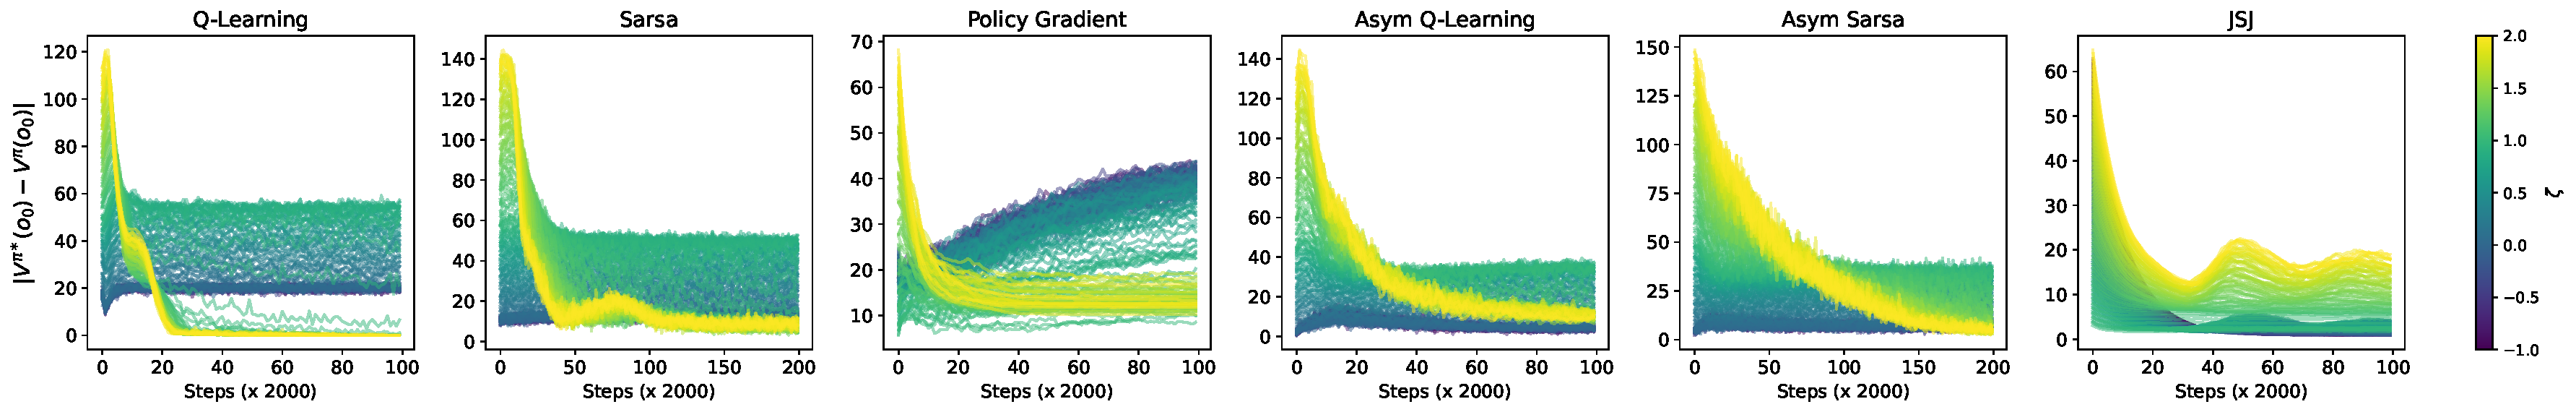
\includegraphics[width=1\textwidth]{images/images_part1/learning_curves.pdf}
    \caption{Baselines learning curves of partially observable policies in POIBMDPs. 
    In each subplot, each single learning curve is colored by the value of $\zeta$ in the corresponding POIBMDP in which learning occurs. 
    Each single learning curve represent the sub-optimality gap averaged over 100 seeds.
    So for each baseline we ran a total of $200 \times 100$ single training run.
    }\label{fig:rl-poibmdp}
\end{figure}

\begin{figure}
    \centering
    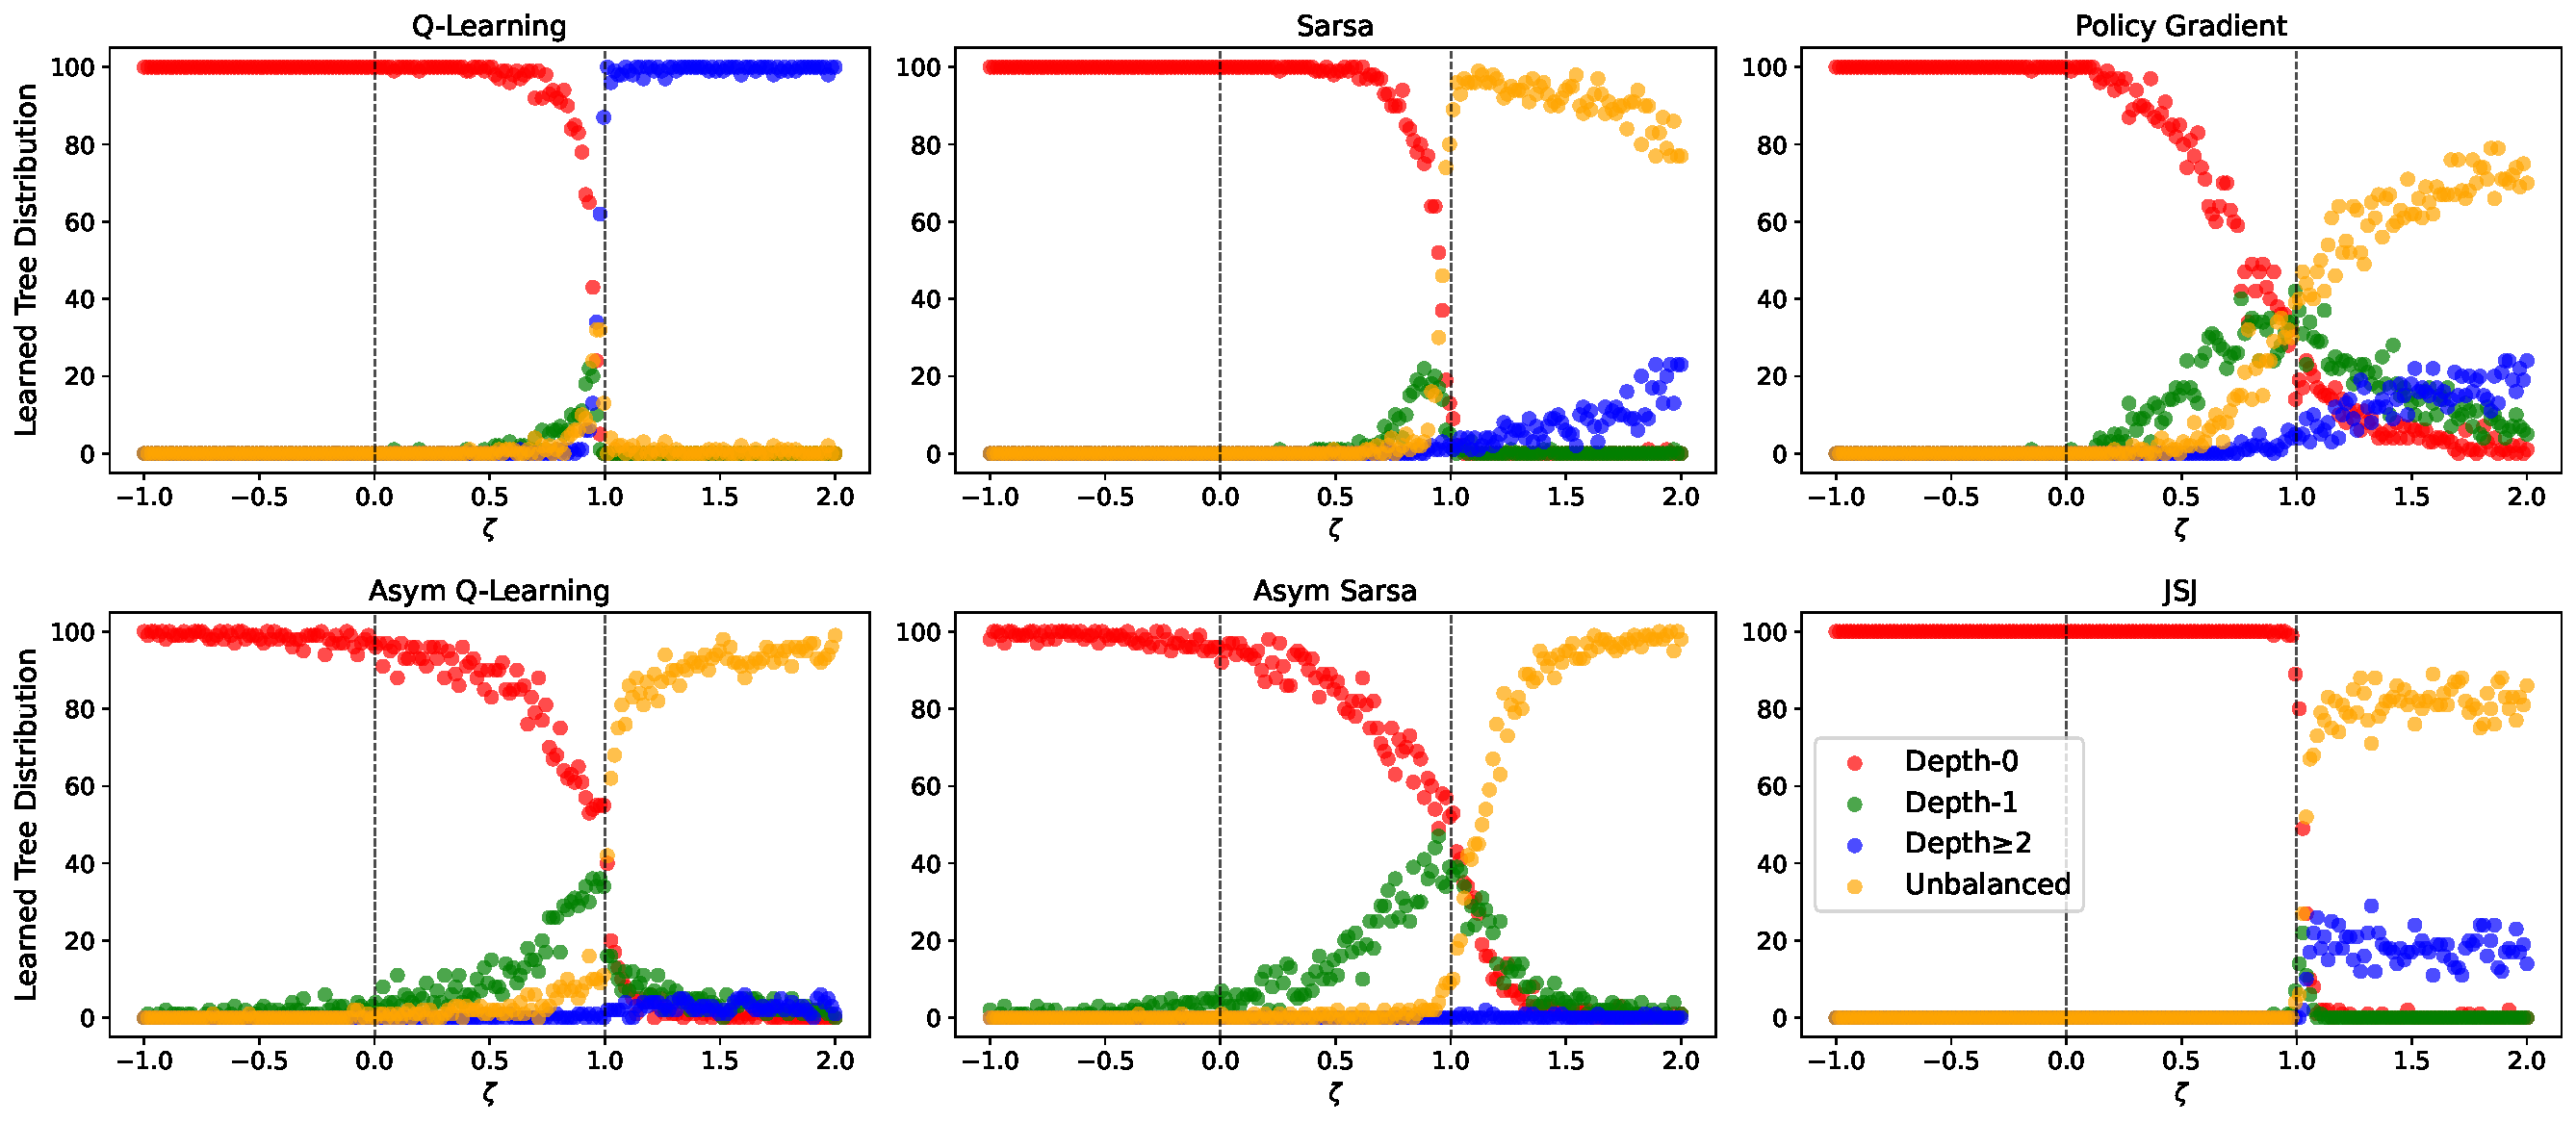
\includegraphics[width=1\textwidth]{images/images_part1/tree_distributions.pdf}
    \caption{Distributions of final tree policies learned across the 100 seeds.
    For each $\zeta$ value, there are four color points each represeting the share of depth-0 trees (red), depth-1 trees (green), unbalanced depth-2 trees (orange) and depth-2 trees (blue).
    Note that those tres do not necessary correspond to tres in Figure (cite). We simply check the structure of trees and not if they are the best-in-class tree. 
    }\label{fig:dt-distrib-poibmdp}
\end{figure}


\subsection{How difficult is it to learn in POIBMPDs?}

As discussed in the previous chapter (cite), POIBMDPs inherit many difficulties from POMDPs.
To prove that solving POIBMDPs, even though there are only a handful of states, observations, and actions (16, 9, and 6 respectively), we compare the success rate of RL baselines when applied to a POIBMDP with $\gamma=0.99$, $\zeta=0.5$ and when applied to the corresponding fully observable IBMDP.
Because we know that for those values of $\zeta$ and $\gamma$, the optimal deterministic partially observable policy is a depth-1 tree and the optimal fully observable policy is a tabular policy from Figure (cite); we can compute the success rate of an RL algorithm as the proportion of learned policies that match their optimal counterparts.

Furhtermore; we also consider advanced tricks for tabular RL in order to properly assess the difficulty of learning in POIBMDPs compared to learning in IBMDPs:
\begin{enumerate}
    \item Optimistic Q-function (cite)
    \item Entropy regularization (cite)
    \item Eligibility traces (cite)
    \item $\epsilon$-decay (cite)
\end{enumerate}
In particular, for each of the aforementioned RL baselines; we learn policies using a wide variety of hyperparamters.
For example, in Table (cite) we provide the detailed hyperparameter space of Asymmetric Sarsa, which induce a total of 1152 instances of Asymmetric Sarsa, and in Table (cite) we provide the hyperparameter space sizes for all baselines 
We run each baseline using each hyperparamters combination 10 times on 1 million timesteps.

\begin{table}[h]
\centering
\caption{Asymmetric Sarsa Hyperparameter Space (768 combinations)}
\begin{tabular}{lll}
\toprule
\textbf{Hyperparameter} & \textbf{Values} & \textbf{Description} \\
\midrule
Epsilon Schedules & (0.3, 1), (0.3, 0.99), (1, 1) & Initial exploration and decrease rate \\
Epsilon Schedules & (0.1, 1), (0.1, 0.99), (0.3, 0.99) & Initial exploration and decrease rate \\
Lambda & 0.0, 0.3, 0.6, 0.9 & Eligibility trace decay \\
Learning Rate $U$ & 0.001, 0.005, 0.01, 0.1 & $Q$ learning rate \\
Learning Rate $Q$ & 0.001, 0.005, 0.01, 0.1 & $U$ learning rate \\
Optimistic & True, False & Optimistic initialization \\
\bottomrule
\end{tabular}
\end{table}

\begin{table}[h]
    \centering
    \caption{Summary of RL baselines Hyperparameter Spaces}
    \begin{tabular}{llr}
    \toprule
    \textbf{Algorithm} & \textbf{Problem} & \textbf{Total Hyperparameter Combinations} \\
    \midrule
    Policy Gradient & PO/IBMDP & 420 \\
    JSJ & POIBMDP & 15 \\
    Q-learning & PO/IBMDP & 192 \\
    Asym Q-learning & POIBMDP & 768 \\
    Sarsa & PO/IBMDP & 192 \\
    Asym Sarsa & POIBMDP & 768 \\
    \bottomrule
    \end{tabular}
    \end{table}


\begin{figure}
    \centering
    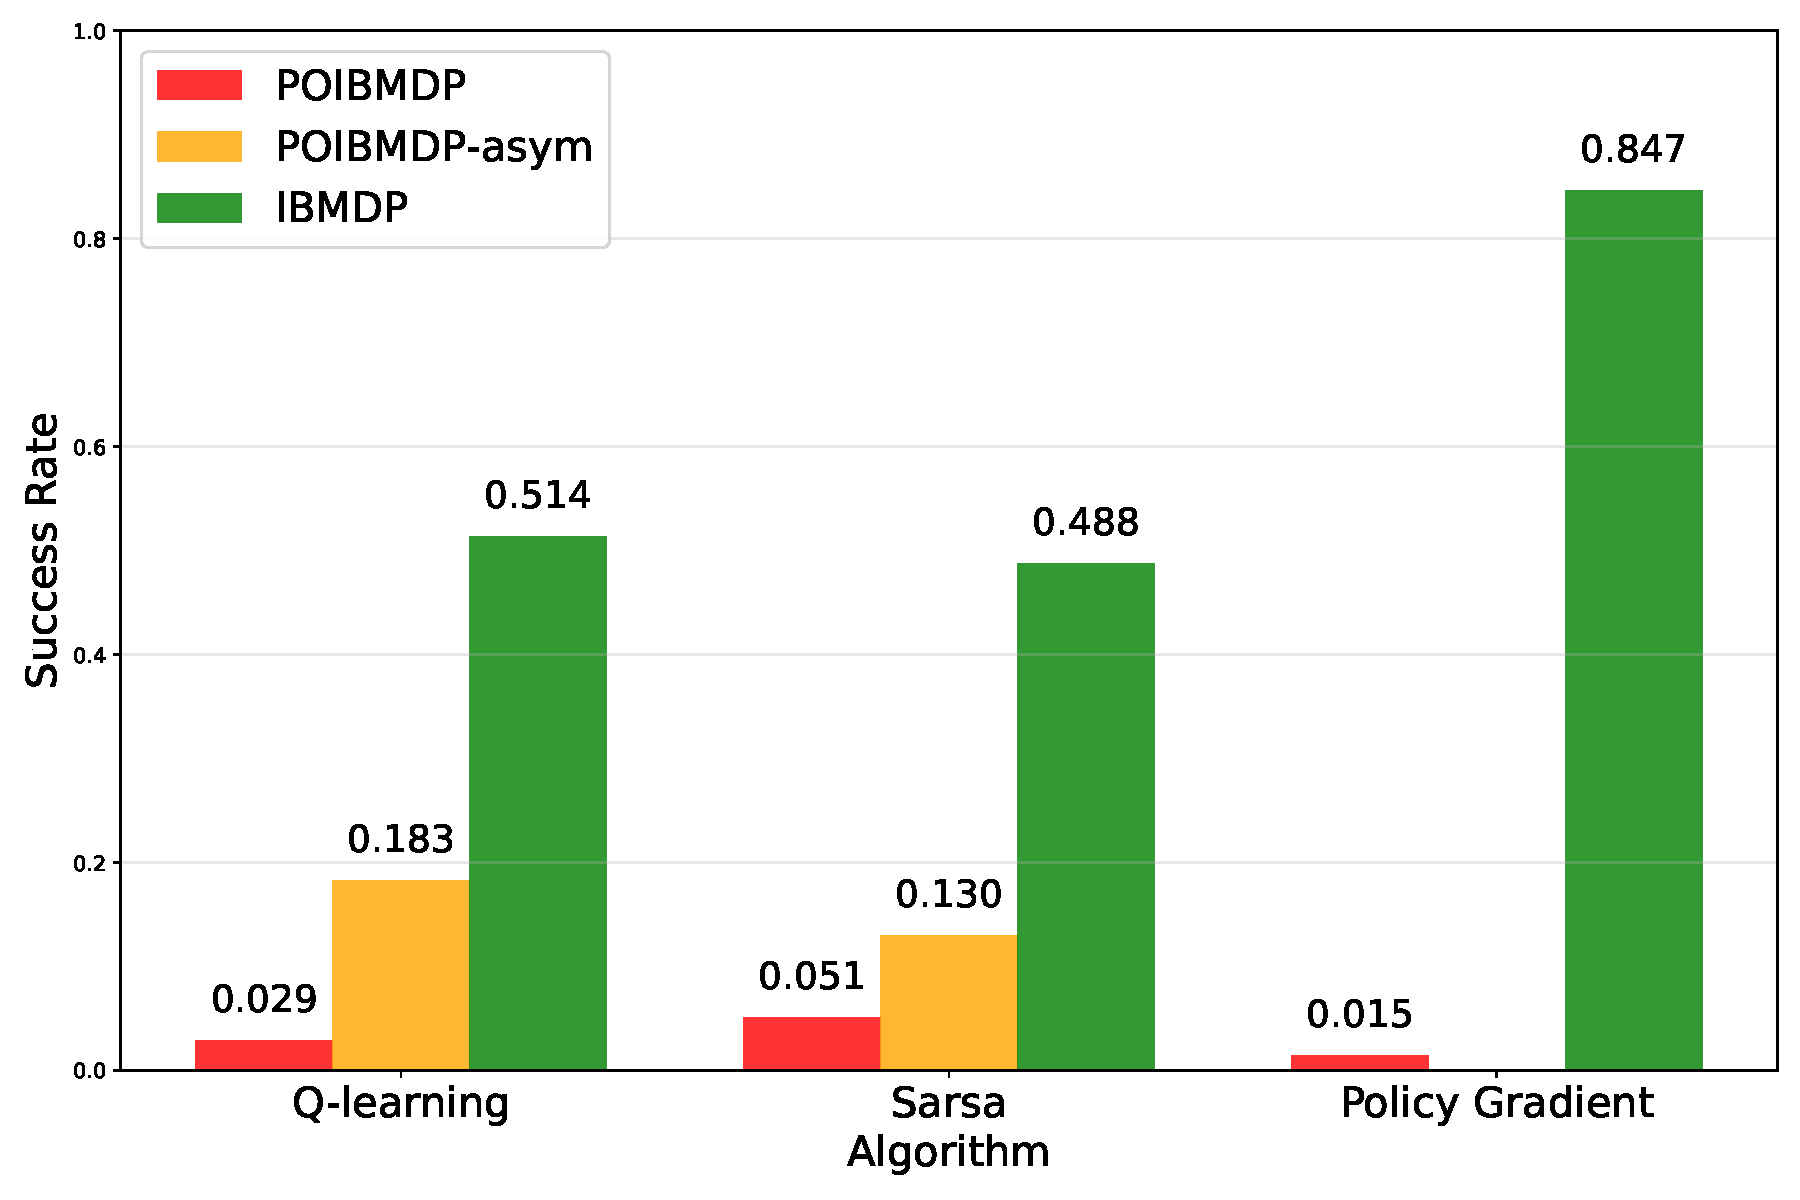
\includegraphics[width=1\textwidth]{images/images_part1/algorithm_performance_comparison_flattened.pdf}
    \caption{Success rates of different RL algorithms over thousands of runs when applied to a POIBMDP and its fully observable IBMDP counterpart}\label{fig:po-vs-ib}
\end{figure}

The key observations from Figure (cite) is that POIBMDPs are way harder than their IBMDPs counterparts.
Even though asymmetry seems to increase performances; learning a decision tree policy for a simple grid world directly with RL using the framework of POIBMDP seem way to difficult and costly as successes might require a million steps for such a seemingly simple problem.
An other difficulty in practice that we did not cover is the choice of information gathering actions.
For the grid world MDP, choosing good IGAs ($x\leq1$ and $y\leq1$) is simple but what about more complicated MDPs? 
Even after choosing candidate IGAs; RL with large action space is known to be an already difficult problem.


\section{[WIP] Reproducing CUSTARD experiments}
In this section, we attempt to reproducie the results from the original IBMDP paper (cite). Authors did not share their code and the description of hyperparameters and algorithms is very light.
\begin{figure}
    \centering
    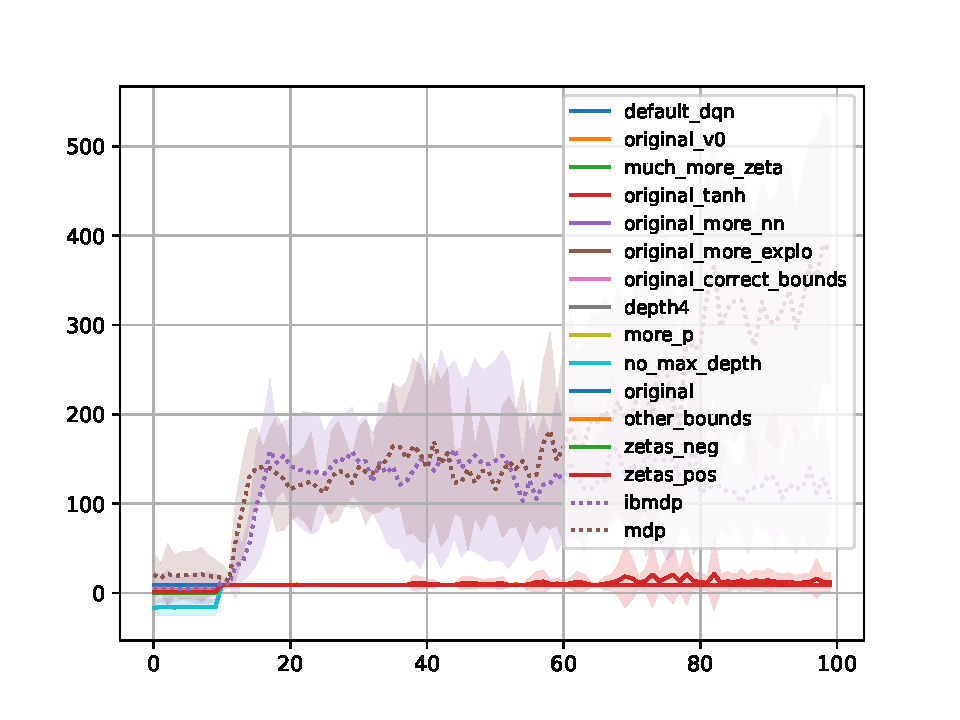
\includegraphics[width=0.8\textwidth]{images/images_part1/test.pdf}
    \caption{Custard (cite) on CartPole.}
\end{figure}

\begin{figure}
    \centering
    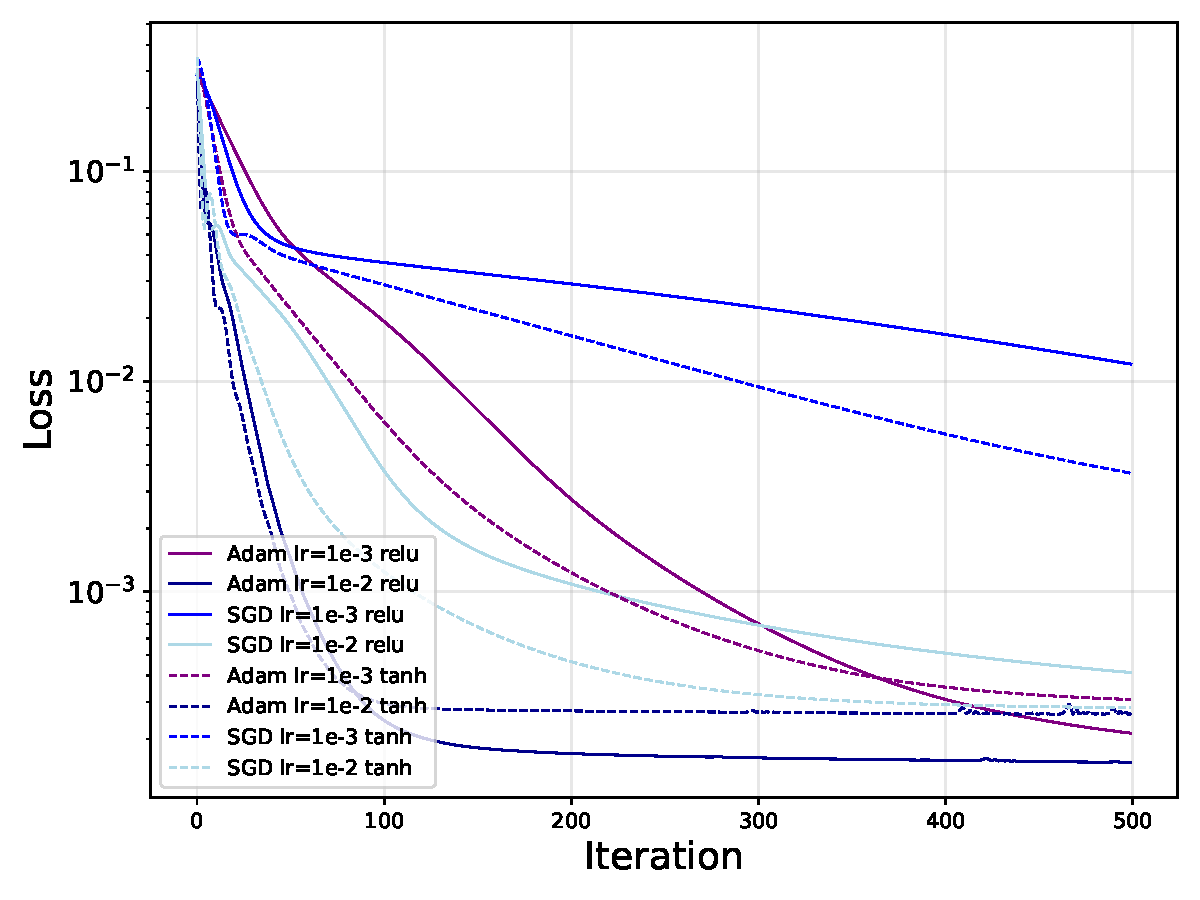
\includegraphics[width=0.8\textwidth]{images/images_part1/repre.pdf}
    \caption{MSE with true $Q^\star(o,a)$ in supervsied setting.}
\end{figure}

\section{Conclusion}
We suggest researchers and practitioners interested in decision tree policies for MDPs to forget about the direct RL approach and focus on the indirect imitation-based approach (cite) that despite being prone to failures too (cite), is cheaper sample and computation wise as one can re-use pretrained expert policies.

If for some reason one has to avoid imitation; fitting parametric trees, trees whose depth and nodes are predifined and where only thresholds are optimized, then one can use SYMPOL (cite) or Soft decision trees (cite).
The latter approach can be beneficial when the user has lots of domain knowledge on what nodes should be in a decision tree policy.

In the next chapter, we show that when the base MDP's transitions are independent of the action, then POIBMDPs are actually \textit{fully} observable which can lead to new decision tree induction for supervised learning.